\setbeamercolor{background canvas}{bg=fitblue}
\begin{frame}
\frametitle{Geometry Shader}
\begin{center}
\Huge {\color{white}Geometry Shader}
\end{center}
\end{frame}
\setbeamercolor{background canvas}{bg=white}

\begin{frame}[fragile]
\frametitle{Geometry shader}
	\begin{itemize}
	\item Geometry shader se nachází za vertex shaderem (za teselací).
	\item Pracuje po primitivech - má přítup ke všem atributům všech vrcholů vstupního primitiva
	\item Umožňuje generování geometrie a její úpravu.
	\item Transformaci bodu na polygon. 
	\item Používá se pro různé efekty (např. stíny (pomocí stínových těles)).
	\item Další využití může být v částicových systémech.
	\item Geometry Instancing.
	\item Transform feedback.
	\end{itemize}
\end{frame}

\begin{frame}[fragile]
\frametitle{Geometry shader - vstupy/výstupy}
	\begin{itemize}
	\item V Geometry shaderu je nutné specifikovat typ vstupního primitiva.
	{\scriptsize
	\begin{minted}[frame=lines]{glsl}
layout(points,invocations=N)in;//vstupni primitivum bude bod
//points, lines, lines_adjacency, triangles, triangles_adjacency
//invocations - kolikrat bude GS spusten na jedno primitivum
	\end{minted}
	}
	\item Také je nutné definovat výstupní primitivum a maximální počet výstupních vertexů.
	{\scriptsize
	\begin{minted}[frame=lines]{glsl}
layout(triangle_strip,max_vertices=4)out;//vystup je sekvence troj.
//points, line_strip, triangle_strip
	\end{minted}
	}
	\end{itemize}
\end{frame}

\begin{frame}[fragile]
\frametitle{Geometry shader - bod na čtverec}
	\begin{figure}[h]
		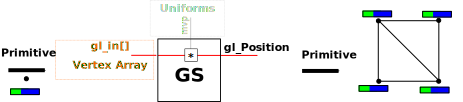
\includegraphics[width=9cm,keepaspectratio]{pics/geometryShader/gs.pdf}
	\end{figure}

	{\scriptsize
	\begin{minted}[frame=lines]{glsl}
#version 430

layout(points)in;
layout(triangle_strip,max_vertices=4)out;

void main(){
  gl_Position=mvp*(gl_in[0].gl_Position+vec4(-1,-1,0,0));
  EmitVertex();
  gl_Position=mvp*(gl_in[0].gl_Position+vec4(-1,+1,0,0));
  EmitVertex();
  gl_Position=mvp*(gl_in[0].gl_Position+vec4(+1,-1,0,0));
  EmitVertex();
  gl_Position=mvp*(gl_in[0].gl_Position+vec4(+1,+1,0,0));
  EmitVertex();
  EndPrimitive();
}
	\end{minted}
	}
\end{frame}

\begin{frame}[fragile]
\frametitle{Geometry shader - fullscreen quad}
	{\scriptsize
	\begin{minted}[frame=lines]{glsl}
#version 430
layout(points)in;
layout(triangle_strip,max_vertices=4)out;
void main(){
  gl_Position=vec4(-1,-1,0,1);EmitVertex();
  gl_Position=vec4(-1,+1,0,1);EmitVertex();
  gl_Position=vec4(+1,-1,0,1);EmitVertex();
  gl_Position=vec4(+1,+1,0,1);EmitVertex();
  EndPrimitive();
}
	\end{minted}
	}
	{\scriptsize
	\begin{minted}[frame=lines]{c++}
glGenVertexArrays(1,&emptyVAO);
//...
glBindVertexArray(emptyVAO);//aktivujeme VAO
glDrawArrays(GL_POINTS,0,1);
glBindVertexArray(0);//deaktivujeme VAO
	\end{minted}
	}
\end{frame}

\begin{frame}[fragile]
\frametitle{shadow volumes - zfail verze}
  \begin{figure}[h]
    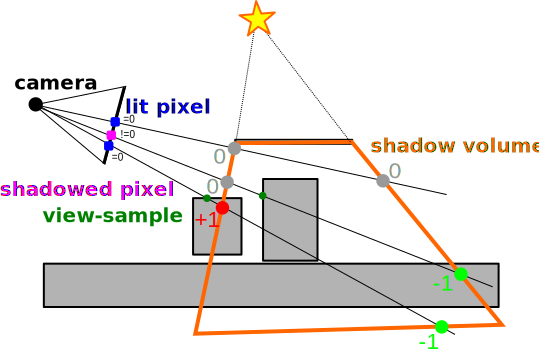
\includegraphics[width=11cm,keepaspectratio]{pics/geometryShader/shadowvolume.pdf}
  \end{figure}
\end{frame}

\begin{frame}[fragile]
\frametitle{Geometry shader - shadow volumes}
  \begin{columns}[T]
    \begin{column}{.44\textwidth}
	    {\tiny
      	\begin{minted}[frame=lines]{glsl}
#version 330
layout(triangles)in;
layout(triangle_strip,max_vertices=10)out;
uniform mat4 MVP,M;//matice
uniform vec4 LightPosition;//pozice svetla
void main(){
  vec4 LP=M*LightPosition;
  vec4 p[6];
  p[0]=gl_in[0].gl_Position;//body trojuhelniku
  p[1]=gl_in[1].gl_Position;
  p[2]=gl_in[2].gl_Position;
  p[3]=vec4(gl_in[0].gl_Position.xyz*LP.w-LP.xyz,0);//v nekonecnu
  p[4]=vec4(gl_in[1].gl_Position.xyz*LP.w-LP.xyz,0);
  p[5]=vec4(gl_in[2].gl_Position.xyz*LP.w-LP.xyz,0);
  vec3 N=normalize(cross((p[1]-p[0]).xyz,(p[2]-p[0]).xyz));
  float Distance=dot(N,LP.xyz)-dot(N,p[0].xyz);
  if(Distance<=0){//otocime volume vnitrkem ven
    vec4 c=p[0];p[0]=p[1];p[1]=c;
    c=p[3];p[3]=p[4];p[4]=c;
  }
  gl_Position=MVP*p[0];EmitVertex();
  gl_Position=MVP*p[1];EmitVertex();
  gl_Position=MVP*p[3];EmitVertex();
  gl_Position=MVP*p[4];EmitVertex();
  gl_Position=MVP*p[5];EmitVertex();
  gl_Position=MVP*p[1];EmitVertex();
  gl_Position=MVP*p[2];EmitVertex();
  gl_Position=MVP*p[0];EmitVertex();
  gl_Position=MVP*p[5];EmitVertex();
  gl_Position=MVP*p[3];EmitVertex();
  EndPrimitive();
}
    	\end{minted}
   	}
    \end{column}
    \begin{column}{.48\textwidth}
	    \begin{figure}[h]
    		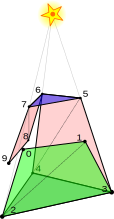
\includegraphics[width=3cm,keepaspectratio]{pics/geometryShader/PerTriangle.pdf}
    	\end{figure}
    \end{column}
  \end{columns}

\end{frame}

